%%%%%%%%%%%%%%%%%%%%%%%%%%%%%%%%%%%%%%%%%
% Thin Sectioned Essay
% LaTeX Template
% Version 1.0 (3/8/13)
%
% This template has been downloaded from:
% http://www.LaTeXTemplates.com
%
% Original Author:
% Nicolas Diaz (nsdiaz@uc.cl) with extensive modifications by:
% Vel (vel@latextemplates.com)
%
% License:
% CC BY-NC-SA 3.0 (http://creativecommons.org/licenses/by-nc-sa/3.0/)
%
%%%%%%%%%%%%%%%%%%%%%%%%%%%%%%%%%%%%%%%%%

%----------------------------------------------------------------------------------------
%	PACKAGES AND OTHER DOCUMENT CONFIGURATIONS
%----------------------------------------------------------------------------------------

\documentclass[11pt]{article} % Font size (can be 10pt, 11pt or 12pt) and paper size (remove a4paper for US letter paper)

\usepackage[utf8]{inputenc} % Set utf8 code
\usepackage[protrusion=true,expansion=true]{microtype} % Better typography
\usepackage[portuguese]{babel}
\usepackage{graphicx} % Required for including pictures
\usepackage{wrapfig} % Allows in-line images
\usepackage[pagebackref]{hyperref}

\usepackage{mathpazo} % Use the Palatino font
\usepackage[T1]{fontenc} % Required for accented characters
\linespread{1.05} % Change line spacing here, Palatino benefits from a slight increase by default

\makeatletter
\renewcommand\@biblabel[1]{\textbf{#1.}} % Change the square brackets for each bibliography item from '[1]' to '1.'
\renewcommand{\@listI}{\itemsep=0pt} % Reduce the space between items in the itemize and enumerate environments and the bibliography

\renewcommand{\maketitle}{ % Customize the title - do not edit title and author name here, see the TITLE block below
\begin{center} % Right align
{\LARGE\@title} % Increase the font size of the title

\vspace{20pt} % Some vertical space between the title and author name

\end{center}
}

\begin{document}

\begin{titlepage}
 \vfill
  \begin{center}
   {\large \textbf{Tiamat}} \\
   {\large \textbf{Void Crawlers}}\\
   {\large \href{mailto:voidcrawlers@gmail.com}{voidcrawlers@gmail.com}}\\[6cm]


   {\Large \textbf{GDD}}\\
   {\Large Versão 0.1}\\[6cm]

   \hspace{.45\textwidth} %posiciona a minipage
  \vfill

\vspace{2cm}

\large \textbf{Brasília}

\large \textbf{Abril de 2015}
\end{center}
\end{titlepage}
\newpage

\tableofcontents

\newpage

%----------------------------------------------------------------------------------------
%	DOC BODY
%----------------------------------------------------------------------------------------

\section{Tabela de Revisão}


\begin{table}[h]
\begin{tabular}{|l|l|p{60mm}|l|}

\hline
\textbf{Versão}  	& \textbf{Data} 	& \textbf{Descrição} 								& \textbf{Autor} 	\\ \hline
0.1               	& 14/04/2015        & Versão inicial              						& Álex Mesquita 	\\ \hline
			      	& 	 	          	&           										&  					\\ \hline
\end{tabular}
\end{table}

\newpage

\section{Objetivo do jogo}

\paragraph{}Jogo singleplayer com temática \textit{Sci-fi}, onde a raça humana vagueia pelo universo a procura de um novo planeta habitável, pois a humanidade extinguiu alguns recursos essenciais que a Terra continha. Após receber um sinal, a raça humana desloca sua nave espacial para um planeta desconhecido a procura desse sinal e acaba encontrando uma torre que definitivamente não podia ter sido construída por humanos. O desafio do jogador será explorar essa torre para descobrir os seus mistérios, porém para isso o jogador deverá explorar o planeta para encontrar recursos que poderão evoluir habilidades dos personagens ou serem utilizados para construir equipamentos para facilitar a exploração da torre.


\section{Visão geral}

\paragraph{}O jogador irá começar o jogo na base de exploração construída próxima a torre a ser explorada. Nesta base haverá algumas construções essenciais para que o jogador possa evoluir os seus personagens, possibilitando assim montar uma estratégia de exploração da torre e dos recursos contidos no planeta.

\paragraph{}A partir da visão de sua base o jogador poderá transitar pelos cenários da torre e da superfície do planeta. Para acessar a torre o jogador deverá clicar sobre um botão de missões na torre que estará disponível no cenário da base, para retornar a sua base o jogador deverá concluir ou abortar a missão. Do mesmo modo para acessar a superfície do planeta o jogador deverá clicar sobre um botão de missões sobre a superfície da torre que também estará disponível no cenário da base, ao abrir o cenário da superfície o jogador poderá selecionar qual missão este irá executar, neste cenário terá um botão para se retornar a base.

\paragraph{}O objetivo do jogo é descobrir quem construiu essa torre tão tecnológica, e ao entrar em contato com tal ser o que ocorreria em seguida? Uma Guerra? Trocas de experiências? Para isso o jogador deverá explorar todos os níveis da torre com os seus personagens. E para facilitar tal exploração será possível coletar \textit{Data points}\footnote{Pontos que serão obtidos através da execução de missões}, podendo assim e evoluir os personagens, facilitando o seu desempenho durante as missões na torre. 

\section{Esquema de controle e interface com o usuário}
Com relação a exploração vertical, dentro da torre, esta será em primeira pessoa, sendo que serão utilizadas as teclas destacadas na figura a seguir:\\
\begin{figure}[!htp]
\centering
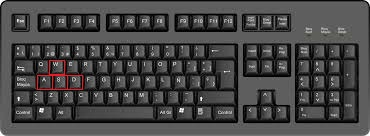
\includegraphics[scale=0.75]{pictures/teclado.jpg}
\caption{Teclas utilizadas}
\label{Teclado}
\end{figure}
\\Onde a tecla ''w'' irá movimentar o jogador para frente, a tecla ''s'' irá movimentar o jogador para trás, a tecla ''a'' irá rotacionar o jogador $90\,^{\circ}$ para a esquerda e a tecla ''d'' irá rotacionar o jogador $90\,^{\circ}$ para a direita.

Com relação a exploração horizontal, na superfície do mundo, o jogador irá usar o \textit{mouse} para navegar na superfície, utilizando o botão direito para selecionar algum objeto e o botão esquerdo para movimentar algum objeto, atacar inimigos e coletar recursos.
\end{document}
